\documentclass[10pt]{article}
\usepackage[margin=0.75in]{geometry}
\usepackage{amsmath,amssymb,booktabs,graphicx,microtype}
\usepackage[hidelinks]{hyperref}
\usepackage[font=small,labelfont=bf]{caption}
\usepackage{enumitem}
\usepackage{placeins}
\setlist{nosep}
\hypersetup{
  pdftitle={Leakage-Safe Soccer Outcome Prediction: Chronological Fine-Tuning, Probability Scoring, and Calibration},
  pdfauthor={M. Law},
  pdfsubject={Final project on reproducible prematch soccer outcome prediction}
}
\title{Leakage-Safe Soccer Outcome Prediction:\
Chronological Fine-Tuning, Probability Scoring, and Calibration}
\author{M. Law\\Final Project Submission}
\date{July 2026}

\begin{document}
\maketitle

\begin{abstract}
We present a reproducible prematch model for three-way soccer outcomes: home win,
draw, or away win. The study normalizes 3,961 match records from StatsBomb Open
Data, constructs 36 features using only information available before each match,
and evaluates logistic regression, random forest, and histogram gradient boosting.
The oldest 80\% of matches form the training period; model and hyperparameter
selection use five expanding-window folds inside that period; and the newest 20\%
remain untouched until final evaluation. Strongly regularized multinomial logistic
regression is selected. On 793 held-out matches from October 2023 through July 2025,
the final model obtains 58.89\% accuracy, 0.9213 log loss, and a 0.5423 multiclass
Brier score, compared with 42.24\%, 1.0644, and 0.6457 for a training-prior
baseline. The apparent accuracy gain is qualified by 49.06\% balanced accuracy,
0.4340 macro F1, and zero hard draw predictions. Temperature scaling chosen from
training-period out-of-fold predictions also worsens held-out log loss by 0.0054.
The result is therefore useful as a reproducible baseline and as evidence that
headline accuracy alone obscures important class and calibration failures.
\end{abstract}

\section{Introduction}

Soccer outcomes are intrinsically probabilistic: team strength, recent form,
venue, rest, and random match events all affect the result. A useful forecast must
therefore be evaluated not only by whether its most likely class is correct, but
also by whether its full probability vector is informative and calibrated.
Probability-sensitive scoring rules are designed for this purpose
\cite{brier1950,gneiting2007}.

This project asks: \emph{how accurately, and with what probability calibration,
can outcomes be predicted from information available before kickoff?} It extends
an earlier prematch random-forest prototype and a separate submission workflow
into one minimal research artifact. The main contributions are:

\begin{enumerate}
  \item a versioned, attributed StatsBomb match table and deterministic feature
  builder whose state is updated only after each current row is emitted;
  \item an evaluation protocol that separates the final chronological holdout
  from expanding-window model selection;
  \item comparison and fine-tuning of three model families using log loss;
  \item accuracy, balanced accuracy, macro F1, log loss, multiclass Brier score,
  confidence calibration, confusion, and permutation analysis; and
  \item machine-readable predictions, cards, hashes, figures, and this paper.
\end{enumerate}

The system is for offline research. It performs no wagering or market action and
uses no audiovisual data.

\section{Data Collection and Provenance}

\subsection{Source}

The input is match metadata from StatsBomb Open Data, whose public repository
provides competition-, season-, and match-level JSON for research and football
analytics \cite{statsbomb}. The inherited local snapshot contains 3,961 completed
matches from 24 competitions between 24 June 1958 and 27 July 2025. The label
distribution is 1,775 home wins (44.81\%), 879 draws (22.19\%), and 1,307 away
wins (33.00\%). Coverage is curated rather than population sampled and varies
substantially by competition, season, era, and gender.

The final repository retains only fields needed for this study: match,
competition, season, and team identifiers; display names; match date; and final
scores. The source and normalized Parquet SHA-256 values begin
\texttt{89690e1c2fbb} and \texttt{1d3243f77e75}, respectively. Their full
64-character values and the schema are recorded in a JSON manifest.

\subsection{Labels and chronology}

For home and away goals $g_h$ and $g_a$, the class is
\begin{equation}
y_i = \begin{cases}
0 & g_h > g_a \quad \text{(home win)},\\
1 & g_h = g_a \quad \text{(draw)},\\
2 & g_h < g_a \quad \text{(away win)}.
\end{cases}
\end{equation}
Rows are sorted by date and match identifier. The first 3,168 rows (through
6 October 2023) are training data; the final 793 rows (7 October 2023 through
27 July 2025) are the test period. Unlike a random split, this setup approximates
forecasting later matches from earlier history.

\section{Prematch Feature Construction}

Each team has state keyed by competition and season. Immediately before match
$i$, the pipeline emits 36 numeric features in five groups:

\begin{itemize}
  \item cumulative matches, wins, draws, losses, goals for and against, and
  points for both teams;
  \item rolling five-match points, mean goals for and against, goal difference,
  and window counts;
  \item home and away Elo ratings and their difference, with initial rating
  1500 and update factor $K=30$ \cite{elo1978};
  \item venue-specific match count, win rate, and goal difference per match; and
  \item capped rest days and the home-away rest difference.
\end{itemize}

For Elo, the expected home score is
\begin{equation}
E_h = \frac{1}{1 + 10^{(R_a-R_h)/400}},
\end{equation}
and the post-match update is $R'_h = R_h + K(S_h-E_h)$, with $S_h$ equal to 1,
0.5, or 0. The key safeguard is ordering: all feature values are read first;
only then are score, rolling, venue, rest, and Elo states updated with the current
result. Automated tests change a current score and confirm that the current
feature vector is unchanged.

State resets at each competition-season boundary. The first appearance of a team
therefore has neutral Elo, zero historical counts, and a 30-day rest sentinel.
Rest values are capped at 30 days to limit long off-season gaps.

\section{Model Fine-Tuning}

\subsection{Candidates}

We compare three probabilistic classifier families:

\begin{itemize}
  \item standardized multinomial logistic regression with
  $C\in\{0.01,0.1,1,10\}$, both with and without balanced class weights;
  \item a 300-tree random forest with maximum depth 6, 12, or unlimited and
  minimum leaf size 1, 5, or 15; and
  \item histogram gradient boosting with $\ell_2$ regularization 0, 1, or 10.
\end{itemize}

The reference baseline is a classifier that always emits the training class
prior; its hard prediction is the training majority class. All stochastic
estimators use seed 42.

\subsection{Selection without test-set reuse}

Model selection uses five expanding-window splits over the 3,168 training rows.
Each validation fold follows its corresponding training fold in time. Candidates
are ranked by mean validation log loss, with accuracy only as a tie-breaker. This
criterion favors useful probability distributions rather than optimizing only
the most likely label. Table~\ref{tab:cv} shows the leading configurations.

\begin{table}[t]
\centering
\caption{Leading expanding-window validation results. Values are fold means;
accuracy and log-loss standard deviations are in parentheses.}
\label{tab:cv}
\begin{tabular}{llll}
\toprule
Model & Parameters & Accuracy & Log loss \\
\midrule
Logistic & $C=0.01$, unweighted & .500 (.076) & 1.009 (.072) \\
Logistic & $C=0.10$, unweighted & .491 (.086) & 1.046 (.116) \\
Random forest & depth 6, leaf 15 & .436 (.088) & 1.048 (.070) \\
Random forest & depth 12, leaf 15 & .440 (.090) & 1.048 (.072) \\
Random forest & unlimited, leaf 15 & .439 (.089) & 1.048 (.073) \\
\bottomrule
\end{tabular}
\end{table}

The selected model is unweighted logistic regression with $C=0.01$, indicating
that strong coefficient shrinkage generalizes better across the heterogeneous
training timeline than more flexible alternatives.

\subsection{Temperature scaling}

To assess post-hoc calibration, the selected candidate generates out-of-fold
training probabilities. A temperature $T\in\{0.50,0.55,\ldots,2.00\}$ is chosen
by minimum log loss on those predictions. Given logits $z$, scaling produces
\begin{equation}
p_k(T) = \frac{\exp(z_k/T)}{\sum_j \exp(z_j/T)}.
\end{equation}
This one-parameter approach follows the temperature-scaling method studied by
Guo et al. \cite{guo2017}. The selected value is $T=1.10$. It is fixed before
the final test probabilities are examined.

\section{Evaluation Metrics}

Accuracy is reported with balanced accuracy and macro F1 because class frequencies
are unequal. For $K=3$ classes, multiclass Brier score is
\begin{equation}
\operatorname{BS} = \frac{1}{n}\sum_{i=1}^{n}\sum_{k=1}^{K}
(p_{ik}-\mathbb{1}[y_i=k])^2,
\end{equation}
and log loss is
\begin{equation}
\operatorname{LL} = -\frac{1}{n}\sum_{i=1}^{n}\log p_{i,y_i}.
\end{equation}
Lower values are better for both proper scores \cite{brier1950,gneiting2007}.
Confidence expected calibration error (ECE) is the count-weighted absolute gap
between mean maximum probability and empirical accuracy in ten equal-width bins.
ECE is descriptive and bin-dependent, so it is considered alongside proper scores.

\section{Results}

\subsection{Held-out performance}

Table~\ref{tab:test} reports the single evaluation on the chronological holdout.
The final scaled model improves accuracy by 16.65 percentage points over the
baseline and reduces log loss by 0.1431 and Brier score by 0.1034. However,
balanced accuracy (49.06\%) and macro F1 (0.4340) are materially lower than raw
accuracy, revealing uneven class performance.

\begin{table}[t]
\centering
\caption{Performance on 793 matches in the untouched 2023--2025 holdout.}
\label{tab:test}
\begin{tabular}{lrrr}
\toprule
Metric & Prior baseline & Unscaled model & Final ($T=1.10$) \\
\midrule
Accuracy & .4224 & .5889 & .5889 \\
Balanced accuracy & .3333 & .4906 & .4906 \\
Macro F1 & .1980 & .4340 & .4340 \\
Log loss & 1.0644 & .9159 & .9213 \\
Multiclass Brier & .6457 & .5389 & .5423 \\
Confidence ECE & .0321 & .0479 & .0652 \\
\bottomrule
\end{tabular}
\end{table}

Temperature scaling is a negative result here. Although $T=1.10$ minimized
out-of-fold training-period log loss (1.0085 versus 1.0091 at $T=1$), it worsened
held-out log loss by 0.0054, Brier score by 0.0035, and ECE by 0.0172. This small
distribution shift illustrates why calibration choices also require temporal
validation and why test-time reversal would be improper.

\subsection{Class behavior and calibration}

Figure~\ref{fig:confusion} is the central failure analysis. The model correctly
classifies 290 of 335 home wins and 177 of 292 away wins, but assigns no match a
draw as its maximum-probability class. Of 166 draws, 105 become home-win and 61
away-win predictions. The model can still allocate nonzero draw probability, so
proper scoring rules retain information not visible in the hard confusion matrix;
nevertheless, a deployment requiring draw identification would be unacceptable.

\begin{figure}[t]
\centering
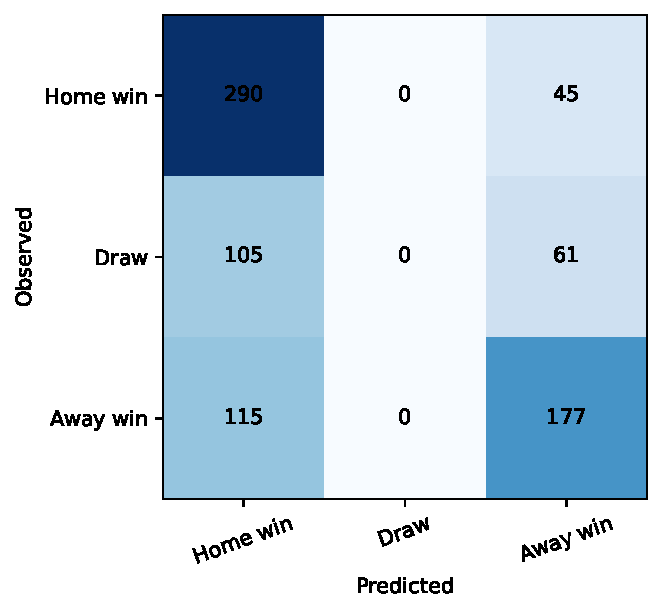
\includegraphics[width=.62\linewidth]{../artifacts/final_run/figures/confusion_matrix.pdf}
\caption{Held-out confusion matrix. The empty draw-prediction column explains the
gap between accuracy and balanced metrics.}
\label{fig:confusion}
\end{figure}

The confidence plot in Figure~\ref{fig:calibration} places most bins above the
diagonal, indicating under-confidence after scaling. The two highest-confidence
bins contain only 25 observations, so their apparent reliability is uncertain.

\begin{figure}[t]
\centering
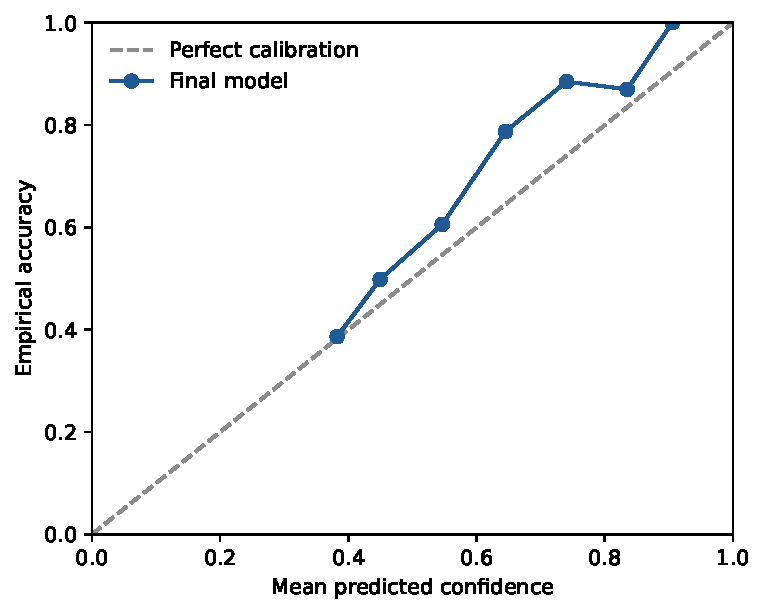
\includegraphics[width=.62\linewidth]{../artifacts/final_run/figures/calibration.pdf}
\caption{Confidence calibration on the chronological holdout. Point sizes are not
weighted; the associated CSV records counts for each bin.}
\label{fig:calibration}
\end{figure}

\subsection{Feature analysis}

Permutation importance on the holdout ranks away five-match mean goals,
home five-match goal difference, home venue goal difference, and Elo difference
as the most influential variables (Figure~\ref{fig:importance}). Importances are
small and correlated predictors can share or mask importance; the plot should not
be interpreted causally.

\begin{figure}[t]
\centering
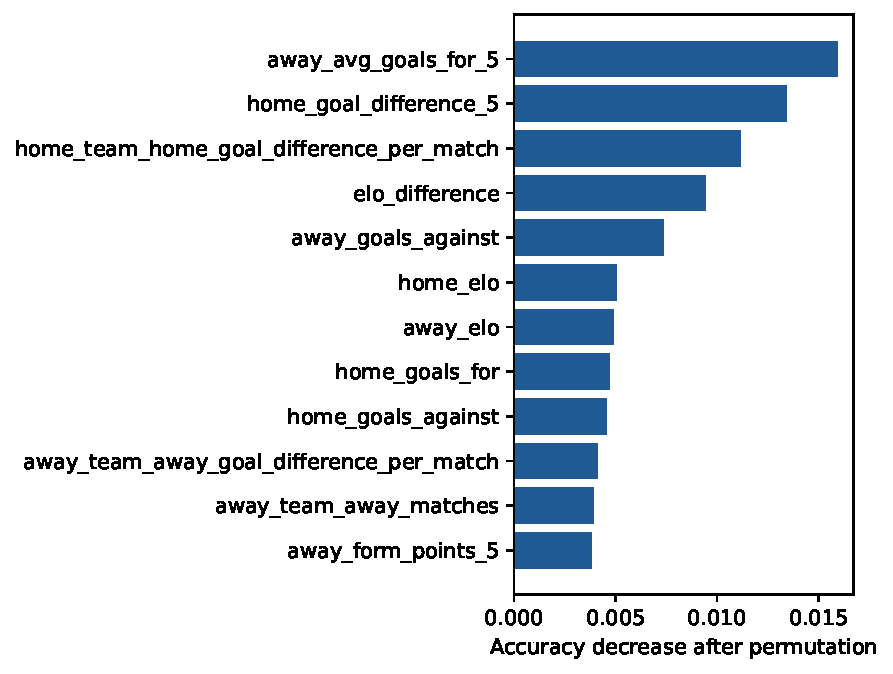
\includegraphics[width=.72\linewidth]{../artifacts/final_run/figures/feature_importance.pdf}
\caption{Top twelve permutation importances, measured as held-out accuracy decrease
after 20 random permutations.}
\label{fig:importance}
\end{figure}

\FloatBarrier

\section{Limitations and Responsible Use}

First, StatsBomb Open Data is curated, so the chronological holdout changes not
only time but its mixture of competitions and seasons. Performance is not a claim
about all soccer. Second, resetting state by competition-season discards continuity
and transfers; cumulative counts can also encode season progress. Third, the model
omits lineups, injuries, coaching changes, market information, and event-derived
expected goals. Fourth, hard draw failure makes raw accuracy incomplete. Fifth,
calibration bins are coarse and the fitted temperature does not transfer cleanly
to the later period. Sixth, permutation analysis is associational.

No model was promoted or connected to decisions. The repository explicitly excludes
real-money use. Any extension should pre-register a later temporal test, improve
draw modeling (for example, ordinal or score-based formulations), quantify uncertainty
across competitions, and test calibration by subgroup.

\section{Reproducibility}

The repository includes normalized input and derived Parquet tables; SHA-256
manifests; Python source; unit tests; all 793 held-out predictions; complete
cross-validation and temperature sweeps; model and data cards; serialized fitted
model; CSV tables; PDF/PNG figures; and the present \LaTeX{} source. The experiment
runs with:

\begin{verbatim}
python -m soccer_final.features
python -m soccer_final.experiment
\end{verbatim}

The recorded run used Python 3.13.12, NumPy 2.5.1, pandas 3.0.5, and scikit-learn
1.9.0 on Apple Silicon macOS. Tests verify leakage ordering and metric utilities.
Artifact hashes allow later readers to distinguish regenerated results from this
submitted run.

\section{Presentation Video Demonstration}

To make the model workflow visible in the final presentation, we built a separate
video demonstration over a 130.33-second, 1920$\times$1080 FIFA highlight clip of
Argentina versus Switzerland. Ultralytics YOLOv8m, pretrained on COCO, detects
persons and sports balls on every second source frame at a 960-pixel inference
size. A transparent HSV jersey-color heuristic labels likely Argentina and
Switzerland players and leaves uncertain detections as generic persons. The ball
was detected on 1,163 of 1,953 sampled frames (59.55\%); 25,090 person and 1,865
ball detections were retained.

The overlay incorporates the submitted prematch model rather than presenting a
disconnected computer-vision demo. Because the versioned training snapshot ends
in 2025, the 2026 fixture has no valid competition-season history. The model is
therefore evaluated at documented neutral new-season state, producing 46.59\%
Argentina, 20.28\% draw, and 33.14\% Switzerland. These fixed values appear under
the larger display. The changing ``current'' visualization adds bounded,
four-second-smoothed evidence from team-colored player confidence and nearest-player
ball proximity in log-probability space. It is explicitly labeled as a research
visualization rather than calibrated betting odds.

Inference ran locally on an Apple M1 Pro with 16 GB unified memory using the
PyTorch MPS backend. The full pass took 146.37 seconds (13.34 sampled frames/s).
A lossless H.264 4:4:4 annotated master was rendered before two-pass delivery
compression. The final 1080p H.264/AAC artifacts are 178.76 MiB for the 200 MB
cap and 44.19 MiB for the 50 MB cap. Both were decoded end to end and visually
checked across wide play, set pieces, close-ups, and the end card. The source clip
declares no downloadable license in YouTube metadata; it is excluded from Git,
attributed on screen, and the derived presentation is documented for local course
use subject to permission and fair-use requirements.

\section{Conclusion}

A carefully regularized linear model provides a strong, auditable baseline for
prematch soccer probabilities: it substantially beats a class-prior baseline on
the later chronological period and outperforms the more flexible candidates during
time-ordered validation. The complete evaluation changes the interpretation,
however. No hard draws are predicted, class-balanced metrics lag raw accuracy, and
training-selected temperature scaling degrades later calibration. The main result
is therefore twofold: leakage-safe form and strength features contain useful signal,
but a credible final project must expose probability and class failures that a single
accuracy number would conceal.

\bibliographystyle{plain}
\bibliography{references}
\end{document}
